\section{Abstract}\label{abstract}

The forensic community depends on datasets containing disk images,
network captures, and other forensic artifacts for education and
research. These datasets must be reflective of the artifacts that
real-world analysts encounter, which can evolve rapidly as new software
is released. Additionally, these datasets must be free of sensitive data
that would limit their distribution. To address the issues of relevance
and sensitivity, many researchers and educators develop datasets by
hand. While this approach is viable, it is time-consuming and rarely
produces datasets that are fully reflective of real-world conditions. As
a result, there is ongoing research into forensic synthesizers, which
simplify the process of creating complex datasets that are free of legal
and logistical concerns.

This work introduces the automated kinetic framework (AKF), a modular
synthesizer for creating and interacting with virtualized environments
to simulate human activity. AKF makes significant improvements to the
approaches and implementations of prior synthesizers used to generate
forensic artifacts. AKF also improves the process of documenting these
datasets by leveraging the CASE standard to provide human- and
machine-readable reporting. Finally, AKF offers several options for
using these features to build and document datasets, including a custom
scripting language. These contributions aim to streamline the
development of forensic datasets and ensure the long-term usefulness of
AKF-generated datasets and the framework as a whole.

\section{Introduction}\label{introduction}

The investigation of cybercrime and other computer-related incidents
requires the collection of forensic datasets, which can broadly be
described as a collection of forensic artifacts. These artifacts are
typically contained in a specific medium, such as a disk image or memory
dump. The accurate collection and analysis of these artifacts are
central to the field of digital forensics; they must be conducted in a
manner that ensures the resulting evidence and conclusions are
admissible in a court of law. Publicly available datasets provide the
artifacts necessary to train new specialists and develop tools to
achieve this goal.

From an education and training perspective, these datasets are critical
in introducing new specialists to the field. Datasets in an educational
setting typically cover a range of techniques and tools, allowing
students to practice applying theoretical concepts learned through
lectures and recitations
\citep{adelsteinAutomaticallyCreatingRealistic2005}. Besides the
specific technical skills covered by these scenarios, these datasets aim
to develop the analytical skills needed for students to adapt to
developments in the field
\citep{cooperStandardsDigitalForensics2010}. In other words, students
should be familiar with standard tools and patterns in digital
forensics, providing a foundation on which more niche techniques can be
learned \citep{lawrenceFrameworkDesignWebbased2009}.

Similarly, from a research perspective, these datasets serve two
purposes. The first is in improving specific processes in the analytic
step of a forensic investigation. Examples include the development of
novel techniques for niche platforms and the improvement of existing,
well-established techniques. The second is in upholding the quality of
the investigation process as new approaches for analyzing datasets are
developed, such as verifying the correctness of automatically carved
files.

There exist various collections of public datasets, such as the Computer
Forensic Reference Datasets (CFReDS) platform
\citep{nationalinstituteofstandardsandtechnologyCFReDSPortal}
maintained by the National Institute of Standards and Technology
(NIST)\footnote{CFReDS is hosted at \url{https://cfreds.nist.gov/}.}.
However, the datasets in these collections are often limited in scope
and realism. In many cases, this can be attributed to privacy and legal
concerns. The sensitive information in real-world datasets limits their
distribution and usage, even if they would otherwise be suitable for
use. As a result, the community often uses \emph{synthetic} datasets,
which are produced specifically for educational and research purposes as
described by Park and Garfinkel et al.
\citep{parkTREDEVMPOPCultivating2018,garfinkelBringingScienceDigital2009}.
However, manually creating these datasets is a time-consuming process
that tends to produce datasets with a very narrow scope and limited
reproducibility
\citep{garfinkelBringingScienceDigital2009,grajedaAvailabilityDatasetsDigital2017}.
It is challenging to develop hands-on labs that realistically and
comprehensively support the ideas learned in theoretical courses
\citep{adelsteinAutomaticallyCreatingRealistic2005,guptaDigitalForensicsLab2022,lawrenceFrameworkDesignWebbased2009}.
Similarly, researchers often have specific needs that are not covered by
existing public datasets, leading to the development of datasets that
are rarely redistributed
\citep{grajedaAvailabilityDatasetsDigital2017}.

There is a clear need for a more streamlined, reproducible method of
developing datasets for research and education -- one that is able to
provide the variability and complex content needed for datasets to be
useful in a wide variety of use cases. One such option is the use of
\textbf{forensic synthesizers}, which aim to automate part or all of
dataset creation by programmatically creating forensic artifacts. Over
the past 15 years, there has been significant research into the
development of these synthesizers, each of which produces artifacts
through distinct approaches. Synthesizers are a subset of broader
automation efforts throughout digital forensics, as described by
Michelet et al. \citep{micheletAutomationDigitalForensics2023}.

Our work, the \textbf{automated kinetic framework}, or \textbf{AKF},
directly improves upon the foundations provided by prior synthesizers to
automate actions that typically require human (``kinetic'') interaction
to perform. It achieves this by adding modern techniques and
technologies to the contributions made by prior synthesizers. In doing
so, it aims to not only vastly reduce the time spent developing new
datasets for research and education, but also improve the documentation
and discoverability of these datasets. Additionally, through AKF's focus
on long-term viability through its modular architecture, educators and
researchers will be able to rapidly develop relevant datasets, even as
new developments and technological advancements occur. Our improvements
are designed to address several challenges observed in prior
synthesizers, specifically the inflexibility of older codebases, the
lack of standardized ground truth, and the difficulty of preparing and
using these synthesizers.

In particular, AKF provides the following novel functionality, each of
which promotes its usage in the broader forensic community.

\begin{itemize}
\item
  \textbf{Significantly simplified library usage and development}: AKF
  uses modern libraries and approaches to greatly simplify the
  implementation of many of its features, including agent communication
  and disk image modification. It also uses technologies such as Vagrant
  to both reduce the difficulty of setting up AKF and improve the
  reproducibility of datasets created by AKF.
\item
  \textbf{Automated dataset documentation in both human- and
  machine-readable formats using the CASE ontology}: Many functions
  throughout AKF generate CASE objects, which document well-known
  artifacts in a structured, queryable format
  \citep{caseyAdvancingCoordinatedCyberinvestigations2017}. We also
  provide functionality to extract the information from supported CASE
  object types and produce a corresponding PDF report. This is supported
  by our custom CASE object definitions, which simplifies use of the
  CASE ontology for Python.
\item
  \textbf{Vastly simplified dataset creation using a custom scripting
  language and AI-assisted workflows}: We provide a YAML-based scripting
  language that provides simplified access to the functionality normally
  exposed by our Python libraries. Additionally, we explore the
  viability of generative AI in creating these YAML scripts, allowing
  datasets to be developed from natural language prompts.
\end{itemize}

This paper begins with an analysis of related work in \autoref{related-work}, covering existing dataset sources and the contributions of prior
synthesizers. In \autoref{artifact-generation}, we introduce AKF's
improvements to creating forensic artifacts by directly modifying disk
images and interacting with virtualized environments. In
\autoref{artifact-documentation}, we then describe how AKF documents
these generated datasets with minimal user overhead, providing both
machine- and human-readable options for identifying artifacts of
interest. Finally, in \autoref{dataset-construction}, we explore how
AKF exposes these artifact generation and documentation features in an
accessible manner, enabling users of all experience levels to benefit
from AKF's design. We conclude with a demonstration and evaluation of
AKF in \autoref{sample-demonstration}, as well as a summary of our work
and future opportunities in \autoref{conclusion-and-future-work}.

\section{Related work}\label{related-work}

We begin with a literature review of two topics relevant to
synthesizers. First, we review existing datasets and the continuing
needs of the field, demonstrating why synthesizers are necessary. We
then cover the specific gaps that these synthesizers have gradually
filled.

\subsection{Existing forensic corpora}\label{existing-forensic-corpora}

Forensic datasets have been available for public use (sometimes upon
request) since the early days of the digital forensics field, although
their sourcing and qualities have changed significantly over time. This
topic was explored in far greater detail by Grajeda et al., who
performed a survey of over 700 research articles to identify the various
datasets used throughout the field
\citep{grajedaAvailabilityDatasetsDigital2017}. However, it is still
important to highlight specific datasets relevant to the development of
synthesizers.

Many early datasets were derived from real sources, such as the used
hard drives collected by Garfinkel from 1998 to 2006, the Enron email
corpus obtained during the federal investigation of Enron, the public
Apache mailing archives, and facial recognition collections
\citep{garfinkelForensicCorporaChallenge2007,grajedaAvailabilityDatasetsDigital2017,yannikosDataCorporaDigital2014,ricanekMORPHLongitudinalImage2006}.
There were also some synthetic datasets developed during this period,
such as the standalone test datasets created by NIST
\citep{woodsCreatingRealisticCorpora2011}. More recent examples
include synthetic datasets produced for the DFRWS Forensics Rodeos and
vendor capture-the-flag (CTF) competitions, such as Cellebrite CTF and
Magnet CTF.

The variety of publicly available forensic datasets increased
considerably in the late 2000s, which can be attributed to both the
overall growth of the field (including the broader field of incident
response) and the advancement of computing as a whole. Various notable
datasets described by Grajeda et al.~include malware samples,
file-specific datasets such as collections of Microsoft Office files,
and datasets for mobile phones. It was also during this time that
non-disk datasets, such as memory dumps and network captures, became
more prevalent. Many of these datasets have been aggregated into
platforms such as Digital Corpora
\citep{garfinkelBringingScienceDigital2009,yannikosDataCorporaDigital2014}
and the NIST CFReDS project, which are actively maintained corpora of
forensic datasets. In 2021, Xu et al.~compiled and published a
repository of educational datasets that explicitly focuses on ease of
use, realism, and breadth \citep{xuDesigningSharedDigital2022}.

These existing datasets are indeed expansive and serve as the basis for
much of the training and research material used today. However, the
field continually requires new datasets that reflect current
advancements in technology, such as updated operating systems or new
applications. For example, instant messaging applications have changed
considerably over the history of the field, ranging from MSN Messenger
in the early 2000s to Skype, Discord, Telegram, Signal, Slack, and more.
Artifacts from these applications must be handled differently, even if
the value of the underlying service to an investigator is practically
the same. Similarly, the strategies for analyzing Windows artifacts have
changed significantly from version to version, as new registry keys
become relevant in analyzing applications while others become unused.

This gradual ``aging'' of datasets, in which their relevance degrades
over time, highlights the continuous need for new datasets. Indeed, the
need for current datasets is one of the reasons identified by Grajeda et
al.~for the manual development of new datasets by research authors; it
was often the case that a modern dataset simply did not exist for their
needs. The datasets throughout this section have demonstrated that many
different kinds of datasets have proved to be relevant in digital
forensics research. It holds that any effort to streamline the
development of forensic datasets should be able to cover as many use
cases as possible without requiring significant changes to the
underlying architecture.

The synthesizers described in \autoref{analysis-of-prior-synthesizers}
have made significant contributions following this principle. For
example, many of these synthesizers have focused on implementing
features that reflect the qualities of real-world datasets. These
features include the ability to execute malware samples in a virtualized
environment, generate network captures, and extract application-specific
artifacts. Also notable is the generation of datasets derived from human
interactions, such as public email distribution lists, photographs of
human faces, and transcripts of conversations. While prior synthesizers
and AKF have not explored this in depth, it is briefly addressed as part
of the generative AI work done as part of AKF in \autoref{generative-ai-workflows}.

\subsection{Analysis of prior
synthesizers}\label{analysis-of-prior-synthesizers}

The functionality and availability of synthesizers have varied
considerably over time. However, the goal of these frameworks has
largely remained consistent: they all aim to reduce the effort required
to produce datasets for research and education. The earliest efforts to
streamline forensic lab development were observed in \textbf{FALCON}
\citep{adelsteinAutomaticallyCreatingRealistic2005} and
\textbf{CYDEST} \citep{bruecknerAutomatedComputerForensics2008},
which aimed to simplify the deployment and evaluation of virtual lab
environments for students.

However, \textbf{Forensig2}, described by Moch and Freiling in 2009 and
revisited in 2012, appears to be the first detailed description of a
forensic synthesizer
\citep{mochForensicImageGenerator2009,mochEvaluatingForensicImage2012}.
Users define scenarios through a Python 2 library that provides
abstractions around various virtual machine (VM) operations, such as
formatting disks, creating partitions, and copying files from the host
to the virtual machine. Artifacts are created through a combination of
disk modifications and interactions with a live QEMU-based VM,
ultimately producing a disk image to be analyzed by students.

The vast majority of later synthesizers are similar to Forensig2 in that
they are all implemented in Python, exposing artifact generation
features to users through a Python library. Notable exceptions include
the \textbf{Digital Forensic Evaluation Test (D-FET)} platform
\citep{buchananCloudbasedDigitalForensics2010}, the
\textbf{Summarized Forensic XML (SFX)} language
\citep{russellForensicImageDescription2012}, and the work described
by \textbf{Yannikos et al.} \citep{yannikosDataCorporaDigital2014}.
These synthesizers use custom languages for creating datasets, providing
alternative abstractions around their functionality.

A summary of the notable aspects of the remaining Python-based
frameworks -- many of which were identified by Göbel et al.
\citep{gobelForTraceHolisticForensic2022} -- is described as follows:

\begin{itemize}
\item
  \textbf{ForGeOSI} \citep{maxfraggMaxfraggForGeOSI2023} introduced
  the use of the VirtualBox SDK to automate various operations (such as
  attaching USB devices and starting video captures), forming the basis
  for much of the work done as part of VMPOP.
\item
  \textbf{ForGe} \citep{vistiAutomaticCreationComputer2015} is
  specifically designed to generate NTFS and FAT32 images, placing data
  directly onto disk images by maintaining and serializing custom data
  structures for supported filesystems.
\item
  \textbf{EviPlant} \citep{scanlonEviPlantEfficientDigital2017}
  encompasses a novel method for efficiently distributing generated disk
  images, which is achieved by generating and distributing differential
  ``evidence packages'' to apply to a base image file. An OS-specific
  injection tool generates relevant artifacts based on the evidence
  package. Since the base image must be downloaded only once, each
  reconstructed disk image is significantly smaller than if distributed
  as a standalone image.
\item
  \textbf{VMPOP} \citep{parkTREDEVMPOPCultivating2018} provides an
  architecture for elaborate VirtualBox control in addition to various
  OS-specific commands. Provided routines for Windows include creating
  restore points, installing programs, mapping network drives, setting
  registry values, and more. Although the architecture as a whole is
  platform-independent, the provided implementations operate with
  VirtualBox and Windows.
\item
  \textbf{TraceGen} \citep{duTraceGenUserActivity2021} is similar to
  VMPOP in that it utilizes the VirtualBox API for various high-level
  operations, but is also like hystck in its use of a Python-based agent
  to carry out application-specific actions.
\item
  \textbf{hystck} \citep{gobelNovelApproachGenerating2020} provides
  routines for automating OS- and application-specific commands through
  both normal Python scripts and YAML configuration files. The framework
  produces network captures and disk images; similar to EviPlant, it
  supports ``differential'' images that can be distributed and applied
  to ``template'' images.
\item
  \textbf{ForTrace} \citep{gobelForTraceHolisticForensic2022} is the
  most recently developed synthesizer, which directly builds upon hystck
  by providing memory captures (alongside disk and network captures) in
  addition to various other new features (such as the ability to execute
  PowerShell scripts to create Windows artifacts), with a focus on a
  modular architecture. A variant focusing on Android artifact
  generation was developed in 2024
  \citep{demmelDataSynthesisGoing2024}.
\end{itemize}

Clearly, significant work has been done to streamline the process of
developing images, although the availability and functionality of each
framework vary greatly. However, except for ForTrace and VMPOP, none of
these synthesizers are direct extensions of prior works, suggesting that
the framework authors' needs could only be met by developing new
frameworks from scratch. While this is not stated in any prior works
(except for hystck \citep{gobelNovelApproachGenerating2020}), the
limited maturity, availability, and maintenance of prior works likely
contributed to the independent development of most synthesizers. For
example, several synthesizers are not open source and thus cannot easily
be extended, as is the case with Forensig2
\citep{mochForensicImageGenerator2009} and TraceGen
\citep{duTraceGenUserActivity2021}. Another reason is that the focus
of certain synthesizers results in an architecture that is simply
incompatible with the goals of newer works. For example, ForGe's
architecture \citep{vistiAutomaticCreationComputer2015} focuses
primarily on direct filesystem manipulation to generate forensic
artifacts and is unsuitable for a synthesizer requiring virtualization.
Similarly, synthesizers that exclusively leverage agentless artifact
generation as described in \autoref{artifact-generation}, such as
VMPOP \citep{parkTREDEVMPOPCultivating2018}, require significant
architectural changes to support agent-based artifact generation.

However, perhaps the largest motivation for constructing new
synthesizers is the lack of ongoing support for virtually all
synthesizers. For the synthesizers that \emph{are} open source, none are
under active development and maintenance, possibly with the exception of
ForTrace. Additionally, the forensic datasets generated by these
synthesizers have not seen significant adoption in either education or
research; many instructors continue to use the human-generated datasets
available on public platforms.

The inflexibility of prior synthesizers, combined with the overall lack
of support and success of synthesizer-based datasets, contributes to the
lack of shared codebases. However, this is not to say that the
individual contributions of prior synthesizers cannot be merged into a
single project that resolves many of the architectural barriers that
have limited the adoption and extension of existing synthesizers. We now
move to a discussion of the three main areas in which AKF makes
significant improvements: artifact generation, artifact documentation,
and dataset creation.

\section{Artifact generation}\label{artifact-generation}

Each of the synthesizers described in \autoref{analysis-of-prior-synthesizers} takes one of three approaches to artifact generation, as
partly described by Scanlon et al.
\citep{scanlonEviPlantEfficientDigital2017}:

\begin{itemize}
\item
  \textbf{Physical}: No virtualization of an operating system occurs
  when generating artifacts; data is written directly to the target
  medium, such as a disk image or virtual hard drive.
\item
  \textbf{Agentless logical}: The synthesizer interacts with a live VM
  to generate artifacts. Interaction is achieved without the need for
  custom software to be installed on the VM; instead, actions are
  achieved using the hypervisor itself or a remote management tool
  native to the virtualized operating system (OS).
\item
  \textbf{Agent-based logical}: The synthesizer interacts with a
  dedicated client, or agent, on a live VM to carry out actions. The VM
  must have the agent installed before any interaction can occur.
\end{itemize}

These three approaches are not mutually exclusive within a single
synthesizer, though many prior synthesizers have supported only one
approach to generate artifacts. \autoref{tbl:prior-techniques} denotes
the approaches used by each of the synthesizers previously discussed.
Where source code is unavailable, a best effort was made to identify the
approach used by a particular synthesizer based on its published paper,
if one exists; otherwise, the entire row contains question marks.


\begin{table*}[tb]
\footnotesize
\centering
\begin{tabularx}{\linewidth}{L{0.2} L{0.2666} L{0.2666} L{0.2666}}
\toprule
  \textbf{Synthesizer} & \textbf{Physical} & \textbf{Agentless} & \textbf{Agent-based} \\
\midrule
  \textbf{FALCON} \citep{adelsteinAutomaticallyCreatingRealistic2005} &
  ? & ? & ? \\
  \textbf{CYDEST} \citep{bruecknerAutomatedComputerForensics2008} & ? &
  ? & ? \\
  \textbf{Forensig2}
  \citep{mochForensicImageGenerator2009,mochEvaluatingForensicImage2012}
  & Yes (filesystem mounting; filesystem-independent editing) & Yes (over
  SSH only) & No \\
  \textbf{D-FET} \citep{buchananCloudbasedDigitalForensics2010} & Yes
  (filesystem mounting; filesystem-independent editing) & No & No \\
  \textbf{SFX} \citep{russellForensicImageDescription2012} & Yes
  (filesystem mounting) & No & No \\
  \textbf{Yannikos et al.} \citep{yannikosDataCorporaDigital2014} & ? &
  ? & ? \\
  \textbf{ForGeOSI} \citep{maxfraggMaxfraggForGeOSI2023} & No & Yes
  (hypervisor interfaces) & No \\
  \textbf{ForGe} \citep{vistiAutomaticCreationComputer2015} & Yes
  (filesystem-aware editing) & No & No \\
  \textbf{ForGen} \citep{jjk422Jjk422ForGen2019} & No & No & No \\
  \textbf{EviPlant} \citep{scanlonEviPlantEfficientDigital2017} & Yes
  (filesystem-independent editing) & No & Yes (unknown mechanism) \\
  \textbf{VMPOP} \citep{parkTREDEVMPOPCultivating2018} & No & Yes
  (hypervisor interfaces) & No \\
  \textbf{hystck} \citep{gobelNovelApproachGenerating2020} & No & No &
  Yes (Python agent) \\
  \textbf{TraceGen} \citep{duTraceGenUserActivity2021} & No & No & Yes
  (unknown mechanism) \\
  \textbf{ForTrace} \citep{gobelForTraceHolisticForensic2022} & No & No
  & Yes (Python agent) \\ \\
\bottomrule
\end{tabularx}
\caption{Summary of artifact generation techniques in prior synthesizers.}\label{tbl:prior-techniques}
\end{table*}


There are advantages and disadvantages to each approach, in addition to
requiring distinct implementation techniques. In this section, we
present our contributions to physical and agentless generation through
our automation library \passthrough{\lstinline!akflib!}\footnote{\passthrough{\lstinline!akflib!}
  is publicly available at \url{https://github.com/lgactna/akflib}.},
which generates artifacts by editing disk images and interacting with
virtual machines.

\subsection{Physical generation}\label{physical-generation}

Physical artifact creation encompasses any technique in which the
virtualization of an operating system is not used to generate artifacts.
This allows the synthesizer to bypass the operating system or related
software that could lead to undesirable non-deterministic behavior. This
is sometimes referred to as \emph{simulating} the creation of artifacts
rather than \emph{virtualizing} their creation.

For example, a scenario developer may want to guarantee that a
particular deleted file is partially overwritten by another file,
ensuring that the deleted file is recoverable from the slack space of
the newly placed file. However, userspace applications are typically
unable to force the reuse of physical disk clusters; they are also
subject to hardware drivers that engage in techniques such as wear
leveling. Physical approaches, which bypass this behavior, can achieve
the desired outcome.

There are three primary techniques for physical artifact planting that
have been implemented by prior synthesizers. These are:

\begin{itemize}
\item
  \textbf{Filesystem mounting}, as done by Forensig2
  \citep{mochForensicImageGenerator2009} and SFX
  \citep{russellForensicImageDescription2012}, in which the
  filesystem is mounted to the host and edited directly.
\item
  \textbf{Filesystem-independent direct editing}, as done by EviPlant
  \citep{scanlonEviPlantEfficientDigital2017}, in which edits to
  specific physical addresses on the disk image are made without any
  parsing or knowledge of the underlying filesystem.
\item
  \textbf{Filesystem-aware direct editing}, as done by ForGe
  \citep{vistiAutomaticCreationComputer2015} and EviPlant
  \citep{scanlonEviPlantEfficientDigital2017}, in which filesystem
  data structures are parsed to determine the physical address(es) of
  the disk image to write to. (It is unclear how EviPlant achieves this,
  as its source code is not available.)
\end{itemize}

AKF supports all three physical techniques to varying degrees; however,
AKF makes the largest improvements in filesystem-aware direct editing.
ForGe \citep{vistiAutomaticCreationComputer2015} implements this by
maintaining NTFS and FAT32 data structures in Python, allowing it to
create a fully virtual representation of these filesystems. This
virtualized filesystem provides ForGe with the information needed to
insert data into known slack and unallocated space while maintaining
filesystem consistency. While extremely powerful, it is inflexible in
two specific aspects:

\begin{itemize}
\item
  ForGe does not provide a generic interface for the filesystems it
  supports. Although the NTFS and FAT32 wrappers provide the same
  methods with identical signatures, this is not strictly enforced by a
  parent class. The lack of a generic interface means that the
  functionality supported across all filesystems is unclear, as is the
  functionality that must be implemented for new filesystems to be
  compatible with ForGe.
\item
  ForGe lacks a ``frontend'' to support arbitrary disk types, regardless
  of the underlying filesystem. ForGe does not support multi-partition
  disks or common non-raw disk formats such as VHD, VMDK, or VDI.
\end{itemize}

Read-only libraries addressing these two issues have been in development
since the introduction of ForGe but have not been integrated into other
synthesizers to achieve the same write capabilities as ForGe. Two such
libraries are \passthrough{\lstinline!libtsk!} (also known as The Sleuth
Kit), the C++ library that powers the open-source digital forensics
software Autopsy \citep{SleuthkitSleuthkit2025}, and
\passthrough{\lstinline!libyal!}, a collection of libraries for
analyzing formats not supported by \passthrough{\lstinline!libtsk!}.
These libraries eventually supported the development of
\passthrough{\lstinline!dfvfs!}, or the Digital Forensics Virtual File
System, a Python library that leverages \passthrough{\lstinline!libtsk!}
and multiple libraries from the \passthrough{\lstinline!libyal!} project
to provide a generic interface for analyzing a variety of disk image
formats and filesystems \citep{Log2timelineDfvfs2025}.

One application of these libraries is in deterministically inserting
data into slack space. AKF uses \passthrough{\lstinline!dfvfs!} to
locate the clusters of a file at a known path in a filesystem, which can
then be used to identify the start of slack space within the file's
clusters (as well as unallocated space in the filesystem). By adding the
physical offset of the cluster within the filesystem to the offset of
the filesystem's partition in the disk image, AKF can write to the exact
location of a file's slack space using the offset-based method described
earlier. This achieves feature parity with ForGe by completely
delegating filesystem- and image-specific details to
\passthrough{\lstinline!dfvfs!}, enabling a filesystem-independent
method for locating slack space.

More generally, this technique provides a deterministic method for
inserting data within the slack space of a filesystem, simulating the
deallocation of a file and its partial replacement with a known file.
However, this does not fully simulate the process of deleting a file
through a running operating system and having a new file replace the
deallocated clusters. In particular, this does not generate OS- or
filesystem-specific artifacts associated with deleting and creating
files; the same applies to other uses of
\passthrough{\lstinline!dfvfs!}, such as simulating data corruption or
inserting data into unallocated space. Future work in the field could
address this gap by combining \passthrough{\lstinline!dfvfs!} with
additional techniques to improve the consistency of physical artifact
generation.

\subsection{Agent-based generation}\label{agent-based-generation}

\textbf{Agent-based artifact creation} involves the use of a dedicated
executable on a VM. This executable serves as an interface between the
host machine and the guest machine. This program runs commands natively
on the VM on behalf of the host machine, accepting commands over a
dedicated network interface. This allows for greater flexibility and
action complexity when compared to agentless approaches. In particular,
it allows application-specific functionality to be implemented using
existing automation frameworks such as Selenium
\citep{SeleniumHQSelenium2025}, Playwright
\citep{MicrosoftPlaywrightpython2025}, and PyAutoGUI
\citep{sweigartAsweigartPyautogui2025}, rather than implementing such
functionality from scratch. For example, Playwright allows us to
flexibly automate complex web browsing actions that prior synthesizers
have often done through hardcoded mouse and keyboard inputs.

Agent-based artifact creation is the approach taken by hystck/ForTrace
\citep{gobelNovelApproachGenerating2020,gobelForTraceHolisticForensic2022},
which refers to its agent as an ``interaction manager.'' Because
ForTrace provides extensive agent functionality and is by far the most
mature synthesizer, AKF's agents borrow heavily from ForTrace's
approach. However, AKF improves upon ForTrace by addressing two specific
implementation issues:

\begin{itemize}
\item
  Commands in ForTrace are sent through a simple string-based protocol.
  In particular, it is challenging to send complex Python objects as
  arguments or return values, as these objects often cannot be easily
  serialized to a string without losing information. An example relevant
  to AKF is passing Playwright browser objects, which contain an
  internal state that is difficult to extract and reconstruct using
  strings alone.
\item
  ForTrace depends on Python's runtime introspection to discover the
  correct modules and functions to call based on the contents of a
  command string, importing these modules during runtime. While this is
  a valid approach, it is more complex than the approach taken by AKF.
\end{itemize}

AKF resolves these issues through the use of RPyC, a library for
symmetric remote procedure calls, for agent communication
\citep{TomerfilibaorgRpyc2025}. Although the RPyC protocol is
symmetric, it is often used in typical client-server architectures to
allow clients to manipulate remote Python objects as if they were local
objects, as well as invoke remote (server) functions using local
(client) parameters. Delegating the serialization and deserialization of
complex objects to RPyC enables us to perform complex operations that
would have been difficult to implement with the simple string-based
protocol of ForTrace.

In ``new-style'' RPyC, this is achieved by running a \emph{service} on
the device where remote operations should be performed. Services expose
a set of functions and attributes that can be accessed remotely by an
RPyC client, doing so by setting up a TCP listener for requests to
access these exposed objects. Clients access these functions and
attributes by name as if they were local objects; arguments passed to
functions are serialized and deserialized in the background, as are the
results of function calls and attribute accesses. These communications
occur over a host-only network interface on the VM, concealing them from
network captures on the Internet-communicating NAT interface.

AKF's application-specific functionality is divided into individual RPyC
``subservices'' created on demand. These subservices implement
automation support for a specific application or group of actions and
are analogous to the agent-side code of individual ForTrace modules. The
agent's main loop is itself an RPyC service responsible for creating and
destroying these subservices upon request. All subservices are known to
this ``dispatch'' service at initialization, eliminating the need for
runtime introspection to find application-specific modules. A high-level
diagram of this design can be seen in \autoref{fig:figure-1}.

\begin{figure*}[htbp]
\centering
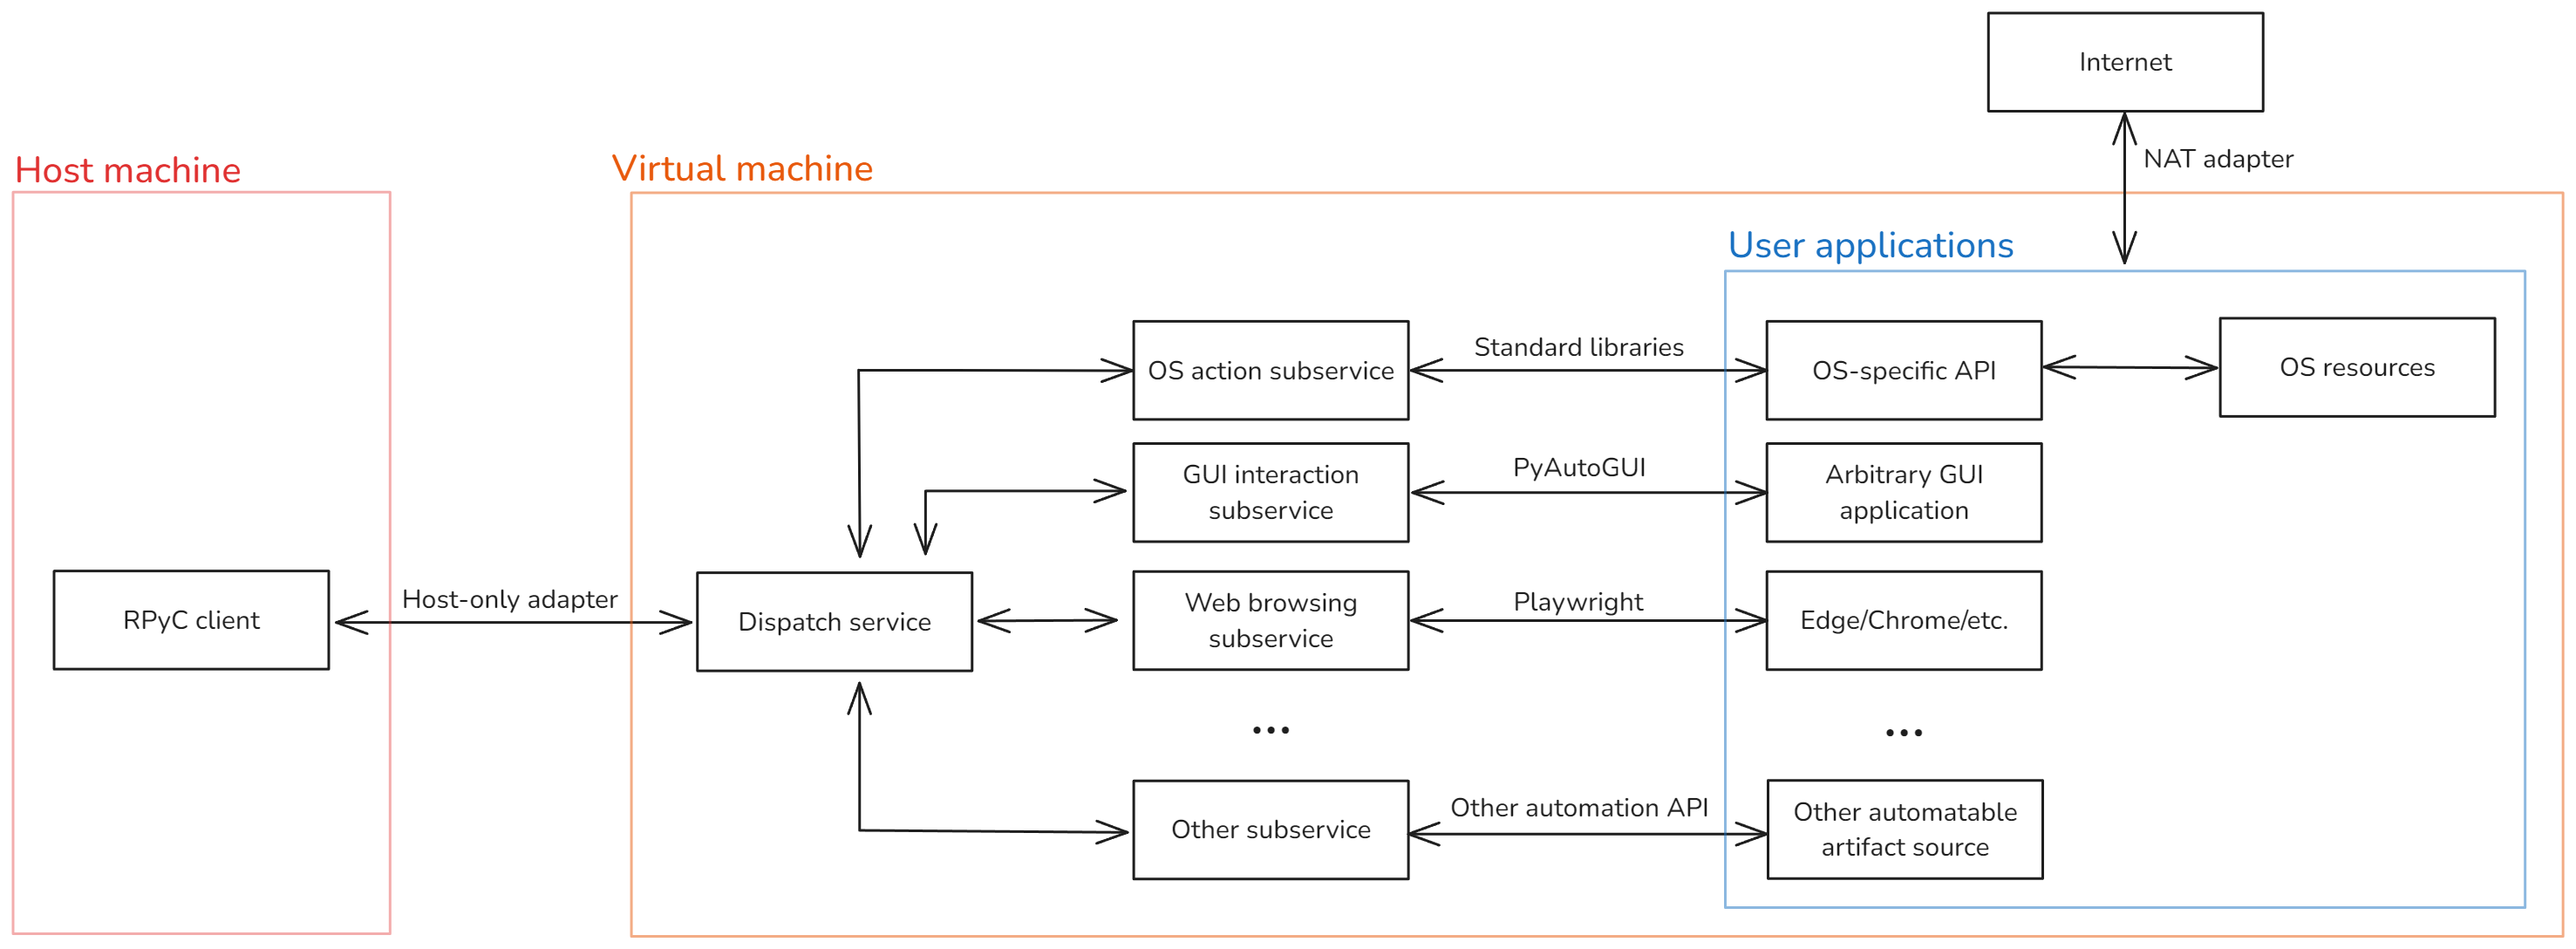
\includegraphics[width=1\linewidth]{figure_1.png}
\caption{Simplified diagram of the AKF agent
architecture.}\label{fig:figure-1}
\end{figure*}

From an implementation and usability perspective, this design provides
three significant improvements over ForTrace. First, the routing of
functions is wholly delegated to RPyC. Instead of manually constructing
a message with the function name and its associated parameters (as
strings) over the network, the process of serializing parameters and
routing them to the correct function call is abstracted away by RPyC.

Second, this allows us to pass and return arbitrarily complex objects
(for which we do not have to manually write the serialization and
deserialization logic). When passing complex objects from the agent to
the server or vice versa, a reference to the object is sent over the
network and wrapped by a \emph{proxy object}, which behaves like the
original object \citep{TheoryOperationRPyC}. Importantly, it is
usually not necessary to distinguish between local and remote/proxy
objects of the same type when writing code, which eliminates the extra
complexity of using proxies.

Finally, the ability to interact with complex remote objects allows us
to significantly reduce the actual code written as part of the API
exposed to the host. For example, there is no need to implement a
wrapper for every method available as part of a Playwright page object;
instead, a reference to the Playwright object \emph{running on the
virtual machine} can be given to the host machine. Instead of writing
individual methods for opening pages, navigating to specific elements,
and so on, we can use the methods that already exist in the Playwright
object -- any local calls on the host's proxy object will lead to remote
outcomes on the virtual machine, as desired. This does not preclude the
ability to write convenience methods for more complex actions requiring
the Playwright object, such as randomly navigating to webpages based on
a provided file containing URLs.

Together, these three features significantly simplify the process of not
only implementing and managing support for individual applications, but
also the actual use of the agent. Simplified application-specific
support makes it easier for the community to extend AKF. Furthermore,
this modular approach to application-specific support enables the
addition or removal of functionality from the agent with minimal effort.
Since not all automation frameworks are available on every platform or
operating system, these ``subservices'' enable us to provide support for
as many different platforms as possible with minimal changes to the
underlying codebase.

\autoref{tbl:akf-comparison} provides brief examples of use cases that
demonstrate how AKF improves upon ForTrace's design.


\begin{table*}[tb]
\footnotesize
\centering
\begin{tabularx}{\linewidth}{L{0.3} L{0.35} L{0.35}}
\toprule
  \textbf{Use case} & \textbf{Implementation in ForTrace} & \textbf{Implementation in AKF} \\
\midrule
  Calling an exposed function in the VM from the host & Manually build a
  valid string containing the name of the function and its serialized
  parameters; implement deserialization and routing logic to correctly
  import and call the corresponding function in the VM. & Call the
  function by name through the RPyC connection using native Python
  objects. Explicit routing logic is not required. \\
  Sending an object from the VM to the host & Extract the internal state
  of the object and convert it to a string (which may not be difficult);
  manually implement deserialization logic that will correctly
  re-instantiate the object based on the extracted state. & All
  serialization logic is already automatically handled by RPyC on both
  ends. Developers typically do not need to add extra logic to transmit
  complex objects. \\
  Expose the methods of a Python object existing on the VM to the host
  machine & Implement wrapper functions for each method to expose on the
  remote object, including logic needed to serialize/deserialize arguments
  on both the host and the VM; this is time-consuming if many methods must
  be exposed. & Expose the Python object directly through RPyC as a
  service attribute; all methods are automatically exposed with no need to
  write individual method wrappers. \\ \\
\bottomrule
\end{tabularx}
\caption{Comparison of the work required to implement certain actions between ForTrace and AKF.}\label{tbl:akf-comparison}
\end{table*}


The list of subservices supported by our AKF agent for
Windows\footnote{The AKF Windows agent, or
  \passthrough{\lstinline!akf-windows!}, is publicly available at
  \url{https://github.com/lgactna/akf-windows}.} is described in
\autoref{tbl:akf-applications}. Although only three subservices are
implemented, each subservice is an example of a distinct design pattern
that could be easily adapted to implement other application-specific
functionality.


\begin{table*}[tb]
\footnotesize
\centering
\begin{tabularx}{\linewidth}{L{0.2} L{0.2} L{0.6}}
\toprule
  \textbf{Subservice} & \textbf{Dependencies} & \textbf{Features} \\
\midrule
  \passthrough{\lstinline!autogui!} & PyAutoGUI
  \citep{sweigartAsweigartPyautogui2025} & Hypervisor-independent mouse
  and keyboard control, as well as other PyAutoGUI features \\
  \passthrough{\lstinline!artifacts!} & Windows-Prefetch-Parser
  \citep{wittPoorBillionaireWindowsPrefetchParser2021} & Collection of
  Windows artifacts and conversion to corresponding CASE objects \\
  \passthrough{\lstinline!chromium!} & Playwright
  \citep{MicrosoftPlaywrightpython2025} & Automated webpage browsing;
  also allows for performing complex actions such as completing forms and
  clicking links based on HTML selectors \\ \\
\bottomrule
\end{tabularx}
\caption{Implemented subservices for the AKF Windows agent.}\label{tbl:akf-applications}
\end{table*}


\section{Artifact documentation}\label{artifact-documentation}

There exists a gap in the ability of instructors and researchers to
perform bulk searches for specific forensic artifacts in public
datasets. For example, the NIST CFReDS repository lacks a unified
standard for describing the artifacts in uploaded datasets. Although
users can search by keywords and human-applied tags, detailed artifact
information is not available in a standardized format that can be
programmatically queried.

For many datasets, an instructor or researcher must read through a PDF
answer key (if one exists) or analyze the image themselves to determine
if a particular artifact is present. Answer keys are not inherently
machine-readable and are not suited for identifying specific artifact
types in bulk. Additionally, the content of human-made reports may be
limited to what the author believes is significant, even if other
artifacts of interest are present in the image. In turn, it may be
difficult to quickly determine if a dataset is useful in demonstrating a
particular technique to students or validating a specific feature of a
newly developed tool.

Given our implementation of artifact generation in \autoref{artifact-generation}, we now address the documentation of these artifacts. This
section describes not only our approach to providing machine- and
human-readable reporting for AKF-generated datasets, but also AKF's role
in providing a foundation for reproducible forensic research.

\subsection{CASE bundles}\label{case-bundles}

A rigid, well-defined format for ground truth is invaluable to
researchers engaging in tool validation and development. We identified
CASE, developed by Casey et al.
\citep{caseyAdvancingCoordinatedCyberinvestigations2017}, as the best
format to meet these needs. CASE is a vendor-neutral format designed to
document both technical and non-technical information about a digital
forensics case. It aims to provide as many definitions as possible for
OS-specific and application-specific artifacts while still providing the
flexibility to describe artifacts from uncommon applications. These
definitions are written in the Terse RDF Triple Language, also known as
Turtle, which expresses object attributes and types in a plaintext
format. Instances of these objects are expressed in a CASE ``bundle,''
which is typically serialized into a format such as JSON-LD.

Because the CASE format itself is language-agnostic, it is necessary to
write language-specific libraries that enable the instantiation of CASE
objects. At the time of writing, the CASE project provides official
Python bindings for CASE version 1.4
\citep{CaseworkCASEMappingPython}. Each unique object type is
represented as a Python class, which can be instantiated to produce
individual objects. However, this library has several limitations,
particularly the need to manually maintain these definitions due to the
instantiation and serialization logic contained in each class.

AKF contributes and leverages its own bindings for CASE\footnote{AKF's
  CASE bindings are publicly available at
  \url{https://github.com/lgactna/case-pydantic}.}. Its foundation is
the Pydantic library for Python, which allows developers to easily
define classes with typed attributes based on Python type hints
\citep{colvinPydantic2024}. This allows us to vastly simplify the
declaration of individual CASE objects while providing runtime type
validation and automatic casting. More importantly, this simplicity
allows us to automatically generate our Python bindings directly from
the Turtle definitions. This is particularly relevant when considering
the active development of CASE version 2.0, which has significant
differences from version 1.4.

Various functions and classes throughout the AKF core libraries and
agent API accept an optional CASE bundle when invoked or instantiated.
As CASE-compatible functions are called, they can automatically add CASE
objects corresponding to the artifacts generated through their
execution. For example, if the agent subservice API for automating
Chromium browser actions is provided with a CASE bundle, navigating to a
page using the subservice API could immediately generate a CASE object
describing the page visit and add it to the bundle. This process can
occur entirely within the host, allowing CASE-related logic to remain
out of the agent when possible.

Other functions are dedicated entirely to creating CASE objects based on
runtime analysis. For example, it is possible to create objects for
Prefetch artifacts as soon as an application is launched. However, these
objects are likely to become outdated if the same application is
launched later in the scenario, thus changing the content of the
prefetch files and making the existing CASE objects inaccurate. To
address this, the \passthrough{\lstinline!artifacts!} subservice
mentioned in \autoref{agent-based-generation} can collect all
Windows prefetch files immediately before a disk image is created,
allowing it to construct CASE prefetch objects that reflect the disk
image without requiring separate tooling. CASE-oriented functionality
can also be implemented in existing subservices; for example, the
\passthrough{\lstinline!chromium!} subservice can also create CASE
objects for Chrome and Edge browser history after all browser automation
actions have been performed. (This is the actual approach taken by the
agent rather than supporting CASE object generation on individual page
visits.)

Sample CASE objects generated by AKF can be seen in \autoref{lst:5.1}.
These CASE objects were part of the full CASE bundle generated as part
of \autoref{sample-demonstration}, and were used to generate the PDF in
\autoref{fig:figure-3}. Both of these CASE objects were generated
immediately before the final disk image was produced (as opposed to
generating them as soon as their corresponding artifacts were created),
as described in the prior paragraph.

\begin{lstlisting}[label={lst:5.1}, caption={Samples of CASE objects contained in the CASE bundle. Note that some JSON elements have been omitted for brevity.}, ]
{
  "@id": "kb:52e6c733-a0f5-4311-907f-0b9e26990e9a",
  "@type": "uco-observable:URLHistoryEntry",
  "uco-observable:url": {
    "@id": "kb:e7584774-49e1-4ecd-bafa-1d247acbcdaf",
    "@type": "uco-observable:URL",
    "uco-core:hasFacet": [
      {
        "@id": "kb:54b7af3b-f1f0-4bb2-95c4-d4fe90d1043c",
        "@type": "uco-observable:URLFacet",
        "uco-observable:fullValue": "https://pastebin.com/2jHBY4R3"
      }
    ]
  },
  "uco-observable:lastVisit": {
    "@type": "xsd:dateTime",
    "@value": "2025-05-26T00:16:33.906+00:00"
  },
  "uco-observable:visitCount": 1,
  "uco-observable:manuallyEnteredCount": 1,
  "uco-observable:pageTitle": "Free Cat Wallpapers - Pastebin.com"
}, ...
{
  "@id": "kb:9cfda173-1ba5-418b-9592-b2593ee88d10",
  "@type": "uco-observable:WindowsPrefetch",
  "uco-core:hasFacet": [
    {
      "@id": "kb:f60d0c57-1375-4838-92e9-ecc118978a79",
      "@type": "uco-observable:WindowsPrefetchFacet", ...
      "uco-observable:lastRun": {
        "@type": "xsd:dateTime",
        "@value": "2025-05-26T00:17:44.162+00:00"
      },
      "uco-observable:timesExecuted": 4,
      "uco-observable:applicationFileName": "BACKGROUNDTRANSFERHOST.EXE",
      "uco-observable:prefetchHash": "a0ec15bd"
    }
  ]
}
\end{lstlisting}

The flexibility of automatic and on-demand CASE object generation makes
it possible to construct CASE objects in a manner that requires little
additional effort from scenario developers. In most cases, scenario
developers do not need to be concerned with instantiating their own CASE
objects when using high-level APIs so long as an AKF library developer
has written support for automatic CASE object construction (and has
documented that this is the case). This significantly reduces the need
for scenario developers to construct ground truth information by
manually analyzing synthesizer-created outputs. When automatic CASE
object generation is not implemented (or different CASE objects are
desired), users can import and instantiate the relevant CASE objects
themselves; these objects can then be manually added to the CASE bundle.

By extension, this means that the detailed documentation of AKF outputs
is innate to many scenarios constructed using AKF. Lowering the effort
required to document an AKF-generated scenario improves the
discoverability and usefulness of all public AKF scenarios to
researchers and educators. This significantly contributes to AKF's goal
of supporting an ecosystem around its images; the CASE bundles of many
scenarios can be queried in bulk to identify datasets that might be
useful for a specific purpose without having to download the dataset
itself. This information can also be used to identify and analyze
broader trends across scenarios, such as the frequency of a particular
artifact appearing in all Windows datasets.

While this machine-readable reporting significantly improves the ability
of the forensic community to locate useful datasets, it is verbose and
unsuitable as a human-readable summary. Human-readable reporting is
particularly relevant in a classroom setting, where the distribution of
simplified answer keys to graders and students focusing on key artifacts
is preferable to the exhaustive reporting provided by a CASE bundle. The
following section addresses the conversion of AKF-generated metadata
into human-readable reports.

\subsection{PDF reporting}\label{pdf-reporting}

Converting a rigid, well-defined format to a human-readable format is
often easier than performing the reverse operation. This is the approach
taken by AKF, which does not create human-readable reports as an
immediate output of artifact generation. Instead, AKF supports a simple
yet flexible system for generating human-readable PDF reports from CASE
bundles produced during artifact generation.

AKF implements human-readable reporting through a set of ``renderers.''
Each renderer accepts a complete CASE bundle and extracts all CASE
objects of a particular type. The renderer then uses the information
contained in these objects to generate a Markdown document, which can
include formatted text, tables, images, and other visual elements. The
results of each renderer are combined to form a larger Markdown document
(or documents) with multiple sections, one for each renderer. The
combined document can be converted to a PDF using Pandoc
\citep{macfarlanePandoc2025}, a general-purpose tool for converting
between documents of various types. Users can modify the generated
Markdown documents before running Pandoc if desired.

A single CASE bundle can be passed through as many or as few renderers
as needed to generate a suitable report for a dataset, as depicted in
\autoref{fig:figure-2}. So long as the original CASE bundle is
available, users can reanalyze datasets with arbitrary renderers; this
means that dataset reports can be regenerated with as much detail as a
user needs for a specific use case. Furthermore, if new renderers are
developed for artifacts that are present in older datasets, the
human-readable report can be regenerated to include these artifacts.

\begin{figure*}[htbp]
\centering
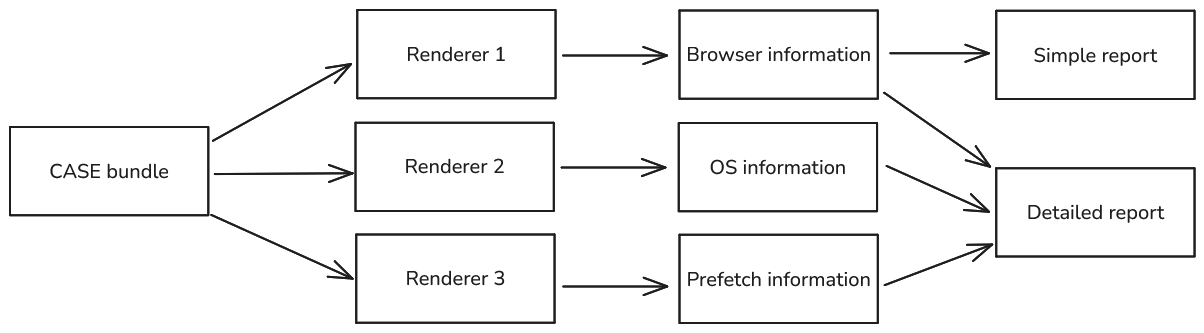
\includegraphics[width=1\linewidth]{figure_2.png}
\caption{Diagram of AKF's modular rendering system.}\label{fig:figure-2}
\end{figure*}

This modular, ``evergreen'' approach to reporting allows these reports
to be interpreted as a focused snapshot of what a dataset contains.
Importantly, this can be done without compromising the dataset itself;
the CASE bundle remains the single, comprehensive source of truth.
Compare this with human-written PDF reports, which may contain human
biases and are rarely maintained in older datasets.

\autoref{fig:figure-3} shows parts of an AKF-generated report for the
sample dataset described in \autoref{sample-demonstration}. Note that
\autoref{fig:figure-3} uses the Eisvogel template
\citep{waglerWandmalfarbePandoclatextemplate2025} for Pandoc,
significantly improving the appearance and readability of generated
documents.

After generating forensic artifacts and any documentation that should be
included with the dataset, the challenge of distributing this
information remains. We now describe our contributions to developing a
format and platform for distributing datasets that are accessible,
reusable, and discoverable.

\subsection{Reproducibility}\label{reproducibility}

A key challenge identified by Grajeda et al.~was the difficulty in
reproducing results in the field of digital forensics. While this is
primarily attributed to the \emph{availability} of forensic datasets in
general, it can also be attributed to challenges in the
\emph{reproducibility} of creating synthetic datasets. Before addressing
the low-level use of AKF as part of \autoref{dataset-construction}, we
will briefly discuss the infrastructure needed to support community
usage of the outputs of AKF scenarios and synthetic datasets as a whole.

There are four elements that must be distributed with a scenario to make
a dataset (and its results) reproducible:

\begin{itemize}
\item
  Any core outputs or individual artifacts generated from the virtual
  machine.
\item
  Any metadata, ground truth, or other reporting that describes the
  scenario.
\item
  The precise instructions required to build the scenario from the
  provided base image, whether human- or machine-readable instructions.
\item
  The OS-specific ``base image'' used to create the dataset, typically a
  virtual machine or disk with a newly installed operating system on
  which all synthesizer actions are performed.
\end{itemize}

The first two have long been a part of many public datasets; however,
less common are detailed instructions to rebuild the dataset from
scratch. A high-level timeline of actions taken, such as that provided
by Woods et al.~in their educational dataset
\citep{woodsCreatingRealisticCorpora2011}, is too imprecise to
guarantee that others will recreate the dataset in the exact same
manner. Non-determinism can be acceptable and even desirable in
education contexts, but it is less desirable for tool validation and
research. Synthesizers, including AKF, provide these instructions
through their machine-readable scripts, which document and execute the
procedure needed to reconstruct a dataset.

However, the distribution of a ``base image'' is perhaps the most
uncommon, even among synthesizers. Besides the extra resources required
to distribute and use virtual disks and appliances, there are also
concerns associated with including copyrighted software, such as Windows
system files. AKF solves this by distributing Vagrantfiles (described in
greater detail in \autoref{setup-and-usage}), which provides a
reproducible method for creating a base image without including
copyrighted content. In doing so, AKF can reliably provide all four
elements noted above, vastly increasing the reproducibility of both the
creation of AKF datasets and any results derived from them.

The inclusion of these elements in a standardized distribution format
could be used to build a distribution platform similar to CFReDS with
more powerful discovery and querying functionality. While CASE enables
queries on a dataset's artifacts, it is also valuable to query the
contents of Vagrantfiles and AKF scripts. For example, a user may want
to search for all images that use the agent-based Chromium artifact
generation described in \autoref{agent-based-generation}, which can be
achieved by searching for the inclusion of the relevant AKF libraries in
the scenario's scripts. Discussed briefly in \autoref{conclusion-and-future-work} is the related challenge of efficiently storing and
distributing these datasets to support such a platform.

It is worth noting that copyright concerns may also apply to the
artifacts themselves, such as disk images and memory dumps that contain
Microsoft executables. Prior educational datasets have addressed this
issue by rendering the OS unbootable
\citep{woodsCreatingRealisticCorpora2011,garfinkelBringingScienceDigital2009},
although this reduces realism. As observed by the authors of TraceGen
\citep{duTraceGenUserActivity2021}, synthesizers alleviate this by
allowing users to distribute only the scripts and base images used to
create a dataset. While this does not guarantee a perfect recreation of
the dataset as intended by the authors (for example, external resources
accessed as part of the scenario can change over time), many artifacts
will likely remain consistent with the original dataset. Thus, the
overall value of the dataset is preserved across different users, even
if the original dataset itself cannot be distributed.

With the reproducibility and value of AKF-generated scenarios
established, we now discuss how to invoke and leverage the underlying
technologies that provide these benefits.

\section{Dataset construction}\label{dataset-construction}

At this point, we have described the functionality for automating
artifact generation in a reproducible manner with comprehensive logging
and reporting. However, there is still the challenge of exposing this
functionality in a user-friendly manner. This section explores the
various improvements AKF makes in simplifying the initial setup process,
writing scripts to create new datasets, and converting abstract ideas
into a coherent script.

\subsection{Setup and usage}\label{setup-and-usage}

Like many of its predecessors, AKF implements its functionality and
exposes its API in Python 3. There are numerous advantages to a
Python-based API; besides the relatively low difficulty of setting up
and using Python, its rich ecosystem allows dataset creation to be
extended through other libraries from the Python ecosystem.

Users must install two foundational technologies for AKF to operate:
Python 3.11 or later and a supported hypervisor (currently, only
VirtualBox). AKF uses \passthrough{\lstinline!pyproject.toml!} to define
Python library dependencies, which can be installed into a virtual
environment using a package manager such as
\passthrough{\lstinline!pip!} or \passthrough{\lstinline!uv!}.

At this point, a virtual machine must be prepared for use with AKF. As
with prior synthesizers, it is possible to manually configure a machine
by downloading a supported operating system and creating a new virtual
machine from scratch. The manual process, similar to that of other
synthesizers, involves installing the operating system, configuring
network interfaces, installing the AKF agent on the device, and then
configuring it to run in the background on startup. The resulting
virtual machine can be cloned and reused for multiple datasets as
needed.

Although relatively straightforward, this process is still
time-consuming, especially when adapted to new operating systems. While
a prepared AKF virtual machine can be distributed in a virtual appliance
format such as OVF, this is not always possible due to the copyright
concerns raised in the previous section. To help resolve this, AKF uses
modern infrastructure-as-code solutions to vastly simplify the setup of
new virtual machines. Vagrant, developed by HashiCorp, is a tool for
rapidly building development environments
\citep{HashicorpVagrant2025}. It allows users to define and build
virtual machines on several virtualization platforms, including
VirtualBox and VMWare. Virtual machines are built by configuring a base
image (called a Vagrant ``box'') according to a Vagrantfile, which
describes hypervisor-specific configuration options and instructions to
configure the machine. The Vagrantfile can be distributed to users,
allowing them to build the same virtual machine as intended by a
scenario author. Notably, Vagrant boxes are often self-contained and do
not require access to vendor resources, such as an update server or
licensing server; this makes them more resilient to loss of support from
vendors.

The AKF Windows agent includes a Vagrantfile for creating a new Windows
11 virtual machine with the agent installed and configured, which can
easily be adapted for other platforms and hypervisors. The
Vagrantfile(s) used to generate a dataset should be included with the
dataset itself to maximize reproducibility, as described in
\autoref{reproducibility}. A robust ecosystem of Vagrant boxes exists
for Linux and Windows, many of which can be retrieved from the Vagrant
public registry \citep{hashicorpHashiCorpCloudPlatform}. When
combined with the flexibility of Vagrant across multiple virtualization
platforms, this can significantly improve the reproducibility and
usability of AKF. It should also be noted that Vagrant can configure and
build virtual environments with multiple machines. For organizations
that can express their environments as Vagrantfiles, it may be possible
for AKF to perform artifact generation at scale, allowing for incident
response datasets that reflect real-world networks and events.

Following setup, developers can build scenarios using the AKF core
libraries (\passthrough{\lstinline!akflib!}) and the API of the
platform-specific agent installed onto the virtual machine (such as
\passthrough{\lstinline!akf\_windows!}). This reflects typical
imperative usage, in which environment setup, artifact generation, and
output generation are handled explicitly through a script executed
through the Python interpreter. A Python script demonstrating web
browsing and disk image creation can be seen in \autoref{lst:6.2a}.

\begin{lstlisting}[label={lst:6.2a}, caption={Example of an imperative AKF scenario.}, language=Python]
from akf_windows.api.chromium import ChromiumServiceAPI
from akflib.core.hypervisor.vbox import VBoxExportFormatEnum
from akflib.core.hypervisor.vbox import VBoxHypervisor
from pathlib import Path

# Instantiate a hypervisor object tied to a specific virtual machine
vbox_obj = VBoxHypervisor("windows-vm")

# Start the virtual machine
vbox_obj.start_vm(wait_for_guest_additions=True)

# Visit a single website
with ChromiumServiceAPI.auto_connect(vbox_obj.get_maintenance_ip()) as chromium_service:
    chromium_service.kill_edge()
    chromium_service.set_browser("msedge")
    page = chromium_service.browser.new_page()
    page.goto("bbc.co.uk")

# Stop the virtual machine
vbox_obj.stop_vm(force=False)

# Export the virtual machine to a disk image
vbox_obj.create_disk_image(
    Path("C:/Users/user/Desktop/windows-vm.raw"),
    VBoxExportFormatEnum.RAW
)
\end{lstlisting}

\subsection{The AKF scripting
language}\label{the-akf-scripting-language}

Although powerful, not everybody needs the flexibility of an imperative
programming language like Python, where the user specifies \emph{how}
artifacts must be created in a step-by-step manner. This brings us to
declarative languages, in which the user only specifies \emph{what}
artifacts must exist in the final dataset, and the synthesizer
determines \emph{how} to generate the artifacts. More precisely,
declarative scripts encapsulate the same functionality that could be
achieved by writing code, but expose this in a simpler format. Similar
concepts can be seen in automation frameworks like Ansible, which allows
users to perform complex actions by writing simple YAML scripts.

In designing the AKF declarative syntax, the declarative syntaxes of
prior synthesizers and unrelated technologies were evaluated. The two
syntaxes that contributed most to the AKF declarative syntax were those
of ForTrace and Ansible. In particular, the modular nature of both
syntaxes was adapted to AKF, as was the overall structure of Ansible's
YAML scripts.

Declarative scripts are comprised of metadata, global configuration, a
set of libraries to import, and individual tasks to execute as part of
the scenario. Each task refers to a single \emph{module} by name,
accepting a dictionary of arguments that determine how the module
behaves. Each module encapsulates some specific functionality, such as
visiting a group of websites or generating a disk image. AKF's
interpreter \passthrough{\lstinline!akf-translate!}, which implements
support for our language, parses the script and does one of two things:

\begin{itemize}
\item
  \textbf{Execution}: When instructed to perform actions directly from
  the declarative script, the interpreter imports AKF core libraries and
  agent APIs to perform the required actions encapsulated by each task.
\item
  \textbf{Translation}: When instructed to translate the declarative
  script, the interpreter generates the equivalent code that
  \emph{would} perform the required actions if executed through a
  standard Python interpreter with the necessary libraries installed.
\end{itemize}

The ability of AKF to both execute and translate declarative scripts
provides significant flexibility to scenario developers. To the best of
our knowledge, prior synthesizers have only supported direct execution
from declarative scripts, which limits the opportunities to use
declarative scripts as a ``starting point'' for writing more complex
imperative scripts. (In fact, the code in \autoref{lst:6.2a} was derived
from the script shown in \autoref{lst:6.3.2a}.) An example of a minimal
AKF scenario, carrying out the same actions as the imperative AKF script
in the prior section, can be seen in \autoref{lst:6.3.2a}:

\begin{lstlisting}[label={lst:6.3.2a}, caption={Example of a declarative AKF scenario.}, ]
name: Minimal scenario
description: Browse to the BBC website and export a disk image.
author: User
seed: "0"
libraries:
  - akflib.modules
  - akf_windows.modules
actions:
  # Start an (existing) VirtualBox machine called "windows-vm".
  - name: Instantiate a hypervisor object tied to a specific virtual machine
    module: vbox_init
    args:
      machine_name: "windows-vm"
  - name: Start the virtual machine
    module: vbox_start_vm

  # Visit a website using Microsoft Edge. A temporary instance of the Chromium
  # subservice API is created for the lifetime of this module.
  - name: Visit a single website
    module: chromium_visit_urls
    args:
      browser: "msedge"
      urls: 
       - "bbc.co.uk"

  # Stop the virtual machine and export the virtual machine to a disk image.
  - name: Stop the virtual machine
    module: vbox_stop_vm
    args:
      force: false
  - name: Export the virtual machine to a disk image
    module: vbox_create_disk_image
    args:
      output_path: "C:/Users/user/Desktop/windows-vm.raw"
      image_format: "raw"
\end{lstlisting}

The execution flow of \passthrough{\lstinline!akf-translate!} itself is
straightforward. Given a path to a YAML script, the interpreter loads
the necessary libraries and configuration keys defined in the file,
instantiating resources accordingly. Then, the interpreter runs each
module under the \passthrough{\lstinline!actions!} key with the provided
arguments and configuration in order, continuing until all actions have
been processed. Modules can read and modify a global state dictionary,
allowing otherwise independent modules to cooperate. This is
particularly useful in allowing for ``outputs,'' such as CASE bundles,
to be passed and gradually constructed across modules. This design
allows for context-aware code generation and action execution.

These modules can be located in any library so long as they can be found
through Python's import system. For example, both
\passthrough{\lstinline!akflib!} and the AKF Windows agent contain their
own declarative module libraries, leveraging functionality specific to
each code repository. All modules in the script are located and stored
at the start of script execution, which allows for validation and
runtime efficiency.

Nearly all externally callable functions in the AKF Python libraries are
currently available through declarative scripting. This includes PDF
report generation, virtual machine interaction, and more. The list of
declarative modules available through \passthrough{\lstinline!akflib!}
and the Windows agent is described in
\autoref{tbl:akf-declarative-modules}. Note that these modules are
referred to by their alias, not their fully-qualified module paths that
are also valid names for the \passthrough{\lstinline!module!} key in the
YAML script.


\begin{table*}[tb]
\footnotesize
\centering
\begin{tabularx}{\linewidth}{L{0.3} L{0.7}}
\toprule
  \textbf{Name} & \textbf{Description} \\
\midrule
  \passthrough{\lstinline!create\_akf\_bundle!} & Creates a new CASE
  bundle for use throughout the declarative scenario. \\
  \passthrough{\lstinline!write\_akf\_bundle!} & Write the contents of the
  currently active CASE bundle to disk as a JSON-LD file. \\
  \passthrough{\lstinline!render\_akf\_bundle!} & Pass the currently
  active CASE bundle through a set of provided renderers and construct a
  valid PDF using Pandoc. \\
  \passthrough{\lstinline!vbox\_init!} & Create a new VirtualBox instance
  bound to a specific virtual machine by name. \\
  \passthrough{\lstinline!vbox\_start\_vm!} & Power on the currently
  active virtual machine. \\
  \passthrough{\lstinline!vbox\_stop\_vm!} & Power off the currently
  active virtual machine. \\
  \passthrough{\lstinline!vbox\_create\_disk\_image!} & Export a disk
  image of the current virtual machine. \\
  \passthrough{\lstinline!artifact\_service\_start!} & Remotely start and
  connect to the subservice responsible for collecting Windows
  artifacts. \\
  \passthrough{\lstinline!artifact\_service\_stop!} & Disconnect from the
  subservice responsible for collecting Windows artifacts. \\
  \passthrough{\lstinline!prefetch!} & Analyze all prefetch files on disk
  and construct their corresponding CASE objects. \\
  \passthrough{\lstinline!chromium\_service\_start!} & Remotely start and
  connect to the subservice responsible for interacting with Chromium
  browsers. \\
  \passthrough{\lstinline!chromium\_service\_stop!} & Disconnect from the
  subservice responsible for interacting with Chromium browsers. \\
  \passthrough{\lstinline!chromium\_visit\_urls!} & Visit one or more URLs
  using a specified web browser. \\
  \passthrough{\lstinline!chromium\_history!} & Collect browsing history
  from a specified web browser and construct their corresponding CASE
  objects. \\ \\
\bottomrule
\end{tabularx}
\caption{Available AKF declarative modules.}\label{tbl:akf-declarative-modules}
\end{table*}


Although these declarative modules provide users with significant
flexibility in \emph{using} AKF itself, there remains the challenge of
building artifacts and scenarios to use with AKF. The following section
addresses this challenge.

\subsection{Generative AI workflows}\label{generative-ai-workflows}

Users of synthesizers must still perform a significant amount of work
when generating individual artifacts. For example, although AKF and
other synthesizers can streamline the process of placing and generating
artifacts, users must still provide some of the artifacts themselves.
For example, if a user wants to include an email chain or other
conversation in the dataset, the user would need to provide the entirety
of the conversation themselves. Such conversations would need to be
consistent with the ``theme'' of a scenario.

This is particularly relevant when adding background noise intended to
emulate benign activity; a real user's device would have many email
conversations irrelevant to a particular scenario and would
significantly contribute to the realism of a synthetic dataset. Existing
datasets, such as the Data Leakage Case produced by NIST, contain many
documents that are not thematically consistent. For example, the
``technical documents'' present in the scenario are actually files from
the general-purpose Govdocs corpora
\citep{garfinkelBringingScienceDigital2009}, with a cover page
denoting their intended role in the scenario.

Recent advancements in AI models have made it significantly easier to
generate text, images, and other media from high-level descriptions that
are consistent with a broader theme. Indeed, this can be used to produce
individual artifacts; generative AI models such as DeepSeek-R1
\citep{deepseek-aiDeepSeekR1IncentivizingReasoning2025} and SDXL 1.0
\citep{podellSDXLImprovingLatent2023} can be used to produce
standalone artifacts that can then be used as part of a dataset. For
example, a large language model (LLM) can be directed to create
technical documentation, email conversations, or image generation
prompts that are related to a corporate espionage scenario, which can
then be used when building a corresponding educational disk image.

However, perhaps a larger challenge is determining the specific actions
that must be performed to create a dataset consistent with some larger
theme. Even with the automation features provided by AKF and the ability
to create individual artifacts through generative AI, it still takes
time to turn an idea into a specific sequence of actions. This is where
AKF's simple, modular declarative scripting language is particularly
powerful. In particular, there are two features of the declarative
syntax that enable this process:

\begin{itemize}
\item
  The role of each module is well-defined and often corresponds
  one-to-one to a specific action that a human might take, such as
  visiting a set of websites.
\item
  The expected inputs for each module are well-defined, as they are
  documented by the required Pydantic argument model for each module.
\end{itemize}

In the same way that declarative scripts are an abstraction around
imperative code, an LLM can be used to facilitate natural language
prompts as an abstraction around creating declarative scripts. To
explore this, we used Ollama to set up a local instance of the
\passthrough{\lstinline!deepseek-r1:32b!} model, interacting with it
through Open WebUI. DeepSeek-R1 was chosen because of its comparable
performance on various benchmarks to proprietary LLMs; the 32 billion
parameter model was chosen as it was the largest model with reasonable
performance on our hardware.

To create AI-generated YAML scripts, we provided our instance of
DeepSeek-R1 with the following information. (The actual prompts and
outputs used to derive the content in this section are included with the
scenario examples in the agent GitHub repository.)

\begin{itemize}
\item
  An overview of the purpose of the declarative syntax.
\item
  The overall structure of the syntax, such as the required top-level
  keys and the structure of individual actions under the
  \passthrough{\lstinline!actions!} key.
\item
  A Markdown-formatted table in which each row contains the name,
  description, and arguments of available modules. Except for the
  arguments column, the table was equivalent to
  \autoref{tbl:akf-declarative-modules}.
\item
  A prompt delimited by \passthrough{\lstinline!<scenario\_prompt>!}
  tags that should be used to build the overall scenario.
\end{itemize}

We observed that this information was generally sufficient for
DeepSeek-R1 to ``understand'' the AKF syntax, allowing it to generate
simple declarative scripts. Although the prompt containing this
information was manually written, much of the prompt could be used as a
template and substituted with the contents of automatically generated
documentation. For example, the table of available modules and their
descriptions could be generated through existing code metadata, such as
the contents of docstrings and Pydantic argument models. Although not
implemented, this use of existing internal documentation is expected to
provide the necessary context for an LLM to function in the future.

In one notable case, DeepSeek-R1 was instructed to create a simple
scenario where a user visited news-related websites with Microsoft Edge
and entertainment-related websites with Google Chrome, ensuring that the
machine underwent multiple power cycles throughout the scenario.
Although DeepSeek-R1 was not provided with examples specific to invoking
the \passthrough{\lstinline!chromium\_visit\_urls!} module, it correctly
constructed an argument dictionary containing several websites that are
thematically consistent for both browsers. It also attempted to use the
\passthrough{\lstinline!vbox\_start\_vm!} and
\passthrough{\lstinline!vbox\_stop\_vm!} actions to perform multiple
power cycles.

However, DeepSeek-R1 sometimes struggled to understand the interactions
between related modules without additional guidance. For example, it did
not infer that the use of the \passthrough{\lstinline!vbox\_stop\_vm!}
and \passthrough{\lstinline!vbox\_start\_vm!} actions required that a
hypervisor instance had been previously created using
\passthrough{\lstinline!vbox\_init!}. Even when the module descriptions
were modified to explicitly state these requirements, it continued to
invoke \passthrough{\lstinline!vbox\_start\_vm!} without a preceding
\passthrough{\lstinline!vbox\_init!} action. In contrast, DeepSeek-R1
appeared to understand that
\passthrough{\lstinline!chromium\_service\_start!} should be called
before calling any other Chromium-related modules, even when this
requirement was not stated. Indeed, the Chromium-related modules
support, but do not require, the use of
\passthrough{\lstinline!chromium\_service\_start!} to explicitly connect
to the Chromium RPyC subservice.

Additionally, DeepSeek-R1 would sometimes invoke modules incorrectly,
such as providing arguments that did not exist or invoking them with the
incorrect name. One notable example was that it incorrectly used
\passthrough{\lstinline!vbox\_start\_vm!} to both start and stop the
virtual machine, adding an erroneous argument when stopping the virtual
machine. In some cases, DeepSeek-R1 deviated significantly from the
declarative syntax and used keys that did not exist, such as specifying
module arguments outside of the \passthrough{\lstinline!args!}
dictionary. Despite these issues related to correctness, it was clear
that DeepSeek-R1 could convert abstract prompts into a sequence of
actions based on the available modules provided. Much like using
declarative scripts as a starting point for imperative scripts, these
outputs can serve as a foundation for more complex declarative scripts.

Furthermore, the issues we identified could be alleviated by providing
additional details to the LLM. For example, AKF developers can extend
the automatically generated documentation provided to the LLM to include
specific examples of module usage, the overall results they cause, and
any constraints on usage. Similarly, users can provide examples of
existing YAML scripts (such as the ones we include in our repositories)
that can help guide the LLM towards accurate use of these modules. In
particular, DeepSeek-R1 is a reasoning model, which means that it
``thinks out loud'' before responding; the model's thoughts could be
used to identify and eliminate vagueness or uncertainty in the provided
prompt. For both users and AKF developers, writing precise prompts and
documentation with this LLM-oriented pipeline could further improve the
quality of generated outputs.

It is important to stress that it remains the user's responsibility to
verify the accuracy and content of AI-generated content. While an LLM
can significantly reduce the time it takes to generate a valid scenario,
it can also produce results that are not consistent with user
expectations. Although errors in ``low-risk'' elements (such as
background noise) may be acceptable, improper use of generative AI with
AKF could lead to datasets that seriously misrepresent real-world
conditions. This significantly impacts the value and integrity of
research and educational material produced through AKF. The CASE and PDF
documentation generated by AKF (as described in \autoref{artifact-documentation}) can be used to help validate that expected artifacts and
dataset qualities are actually present, though it must be complemented
with a broader human evaluation of AI-generated outputs.

Further research is needed to identify common pitfalls when generating
AKF scenarios and individual artifacts through AI, as well as best
practices for similar research- and education-related AI workflows
throughout digital forensics.

\section{Sample demonstration}\label{sample-demonstration}

\subsection{Scenario overview}\label{scenario-overview}

To demonstrate several of AKF's features and the value of an
AKF-generated dataset, we will now explore a simple scenario in which a
user visits websites, saves photos, and then downloads and runs
``ransomware.'' This ransomware simply encrypts the contents of the
Downloads folder before sending the key details and a unique identifier
to a remote web server over HTTP. The ransomware was written in Python
and bundled into an executable using PyInstaller. It was then uploaded
publicly to Google Drive, with the share link posted on an unlisted
Pastebin note.

As part of this scenario, we generated a disk image, network traffic
capture, and a memory dump. These contain the information needed to both
understand how the ransomware was downloaded and reverse the encryption
performed by the ransomware. The scripts and other resources used to
construct this dataset are included in the repository for the AKF
Windows agent\footnote{\url{https://github.com/lgactna/akf-windows/tree/main/scenarios/fsidi}}.
These can be used to reproduce the results described in this section.

To prepare a suitable virtual machine for this scenario, we used a
Vagrantfile to automate the process of creating and configuring a
Windows 11 VirtualBox machine with the AKF agent installed. We
configured two network adapters for the machine: a NAT adapter connected
to the internet and a host-only adapter for communicating with the
agent. We then enabled packet capturing over the NAT adapter, which
would allow us to capture the key sent by the ransomware. Finally, we
created a CASE bundle for use throughout the scenario, which will
include some of the relevant artifacts generated as part of this
dataset.

Once the machine was turned on, we directed the agent to visit a series
of posts on the Reddit platform according to a predefined list of URLs.
This was done by using the Chromium subservice, which uses Playwright to
interact with webpages. For each post, we saved a screenshot of the page
to the Downloads folder, which the ransomware would later encrypt. After
visiting several Reddit posts, we had the agent navigate to and download
the ransomware. We then used the PyAutoGUI subservice to run the
ransomware in File Explorer using a sequence of keystrokes, emulating
how a human would normally run the ransomware. Shortly after, we created
a memory dump of the machine (with the ransomware process still
running), then turned the machine off and created a raw disk image of
the machine. The CASE bundle, along with a PDF report detailing the
bundle's contents, was also exported. Relevant sections of the PDF
report can be seen in \autoref{fig:figure-3}.

\begin{figure}[htbp]
\centering
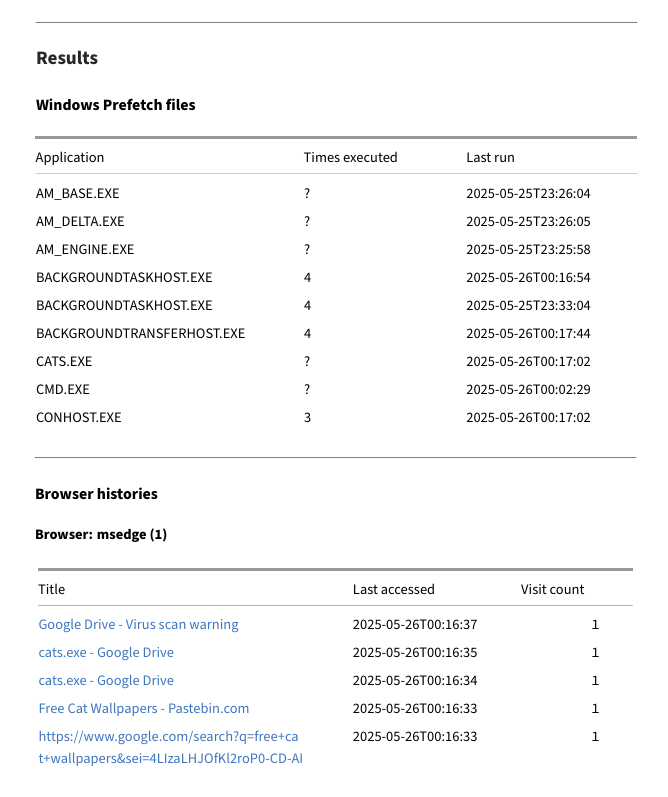
\includegraphics[width=1\linewidth]{figure_3.png}
\caption{Two sections from the AKF-generated PDF
report.}\label{fig:figure-3}
\end{figure}

\subsection{Analysis}\label{analysis}

Now, we turn to a manual analysis of the generated dataset. As part of
this, we will establish the following:

\begin{itemize}
\item
  That the generated artifacts are consistent with the actions specified
  in the script.
\item
  That the generated artifacts are consistent with the documentation
  generated by AKF (when analyzed using external tools).
\item
  That it is possible to reverse the operations performed by the
  ransomware by utilizing multiple aspects of the dataset, specifically
  the disk image, memory dump, and network capture.
\end{itemize}

First, we wanted to verify that the web browsing artifacts were
consistent with the list of URLs specified in the script. We began by
extracting the SQLite database used to store Microsoft Edge browsing
history and viewed the \passthrough{\lstinline!urls!} table containing
browsing history, as shown in \autoref{fig:figure-4}. Indeed, the
entries of the History file are consistent with the URLs specified, as
well as the links shown in the PDF report in \autoref{fig:figure-3}. By
extension, they are also consistent with the JSON-serialized CASE
bundle.

\begin{figure}[htbp]
\centering
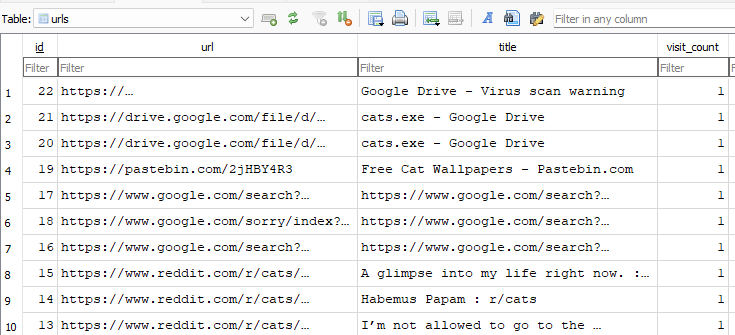
\includegraphics[width=1\linewidth]{figure_4.png}
\caption{The contents of the Microsoft Edge SQLite database in the
sample dataset.}\label{fig:figure-4}
\end{figure}

We also used Eric Zimmerman's PECmd tool to analyze the prefetch entries
contained in the disk image, allowing us to verify the results
documented in the generated PDF (and the CASE bundle). As expected, both
indicate that our ransomware was run, as was Microsoft Edge. More
generally, we noted that although the run times and actual executable
names were consistent, the execution counts recorded by AKF were not.
This may be explained by the differences in the libraries used by PECmd
and our agent subservice.

It is worth noting that several artifacts contained in the Microsoft
Edge database and the Prefetch folder are specific to AKF. These
synthesizer-specific artifacts are discussed in \autoref{discussion}.

To demonstrate the value of each part of the dataset in a digital
forensics, incident response, and reverse engineering context, we will
now decrypt the contents of the Downloads folder using only the data
provided in the dataset. This process involves many skills that are
characteristic of a good educational dataset.

First, we can observe that the ransomware is still present in the disk
image located in the user's Downloads folder. The compiled Python
bytecode can be extracted using a tool such as pyinstxtractor
\citep{extremecodersExtremecodersrePyinstxtractor2025}, which can
then be passed to a bytecode decompiler such as PyLingual
\citep{wiedemeierPYLINGUALPerfectDecompilation2024}. Upon
decompilation, we can determine the mechanism by which files are
encrypted, as well as the information required to decrypt them. Analysis
reveals that the key information is generated randomly at runtime and
then forwarded to a remote server.

To retrieve the information necessary for decryption, we can analyze
either the packet capture or the memory dump independently. If we choose
to analyze the packet capture, we can search for the domain requested by
the ransomware, as indicated in the decompiled code. Doing so reveals
the exact parameters required to reconstruct the key, as shown in
Wireshark in \autoref{fig:figure-5}.

\begin{figure}[htbp]
\centering
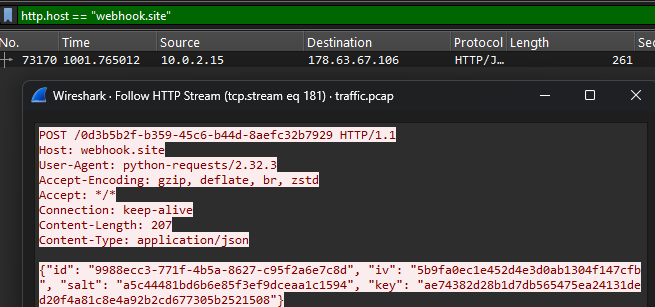
\includegraphics[width=1\linewidth]{figure_5.png}
\caption{The ransomware's web request as seen in the packet
capture.}\label{fig:figure-5}
\end{figure}

Similarly, we can search the memory dump for the key information. Using
a tool such as the Volatility framework or a hex editor, we can analyze
the dump to discover the same JSON in memory as seen in the packet
capture. \autoref{fig:figure-6} depicts the JSON as seen in a hex
editor.

\begin{figure}[htbp]
\centering
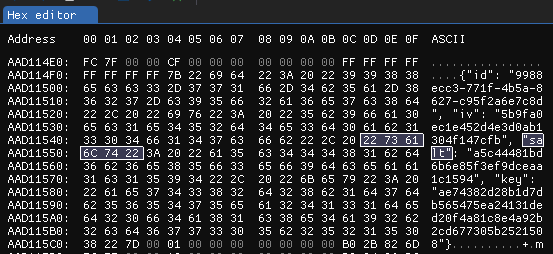
\includegraphics[width=1\linewidth]{figure_6.png}
\caption{The ransomware's web request as seen in the memory
dump.}\label{fig:figure-6}
\end{figure}

At this point, a decryption program can be written based on the
decompiled ransomware logic. To demonstrate that the information
contained in the dataset is sufficient to write a decryption script, we
provided the decompiled ransomware to OpenAI's GPT-4o model and asked it
to produce a decryption script. The resulting script, after
simplification, was successfully used to decrypt the contents of the
Downloads folder. This script is included with our dataset. Note that an
online LLM is used solely to aid in the reproducibility of our analysis;
public models should not be used to analyze confidential datasets.

\subsection{Discussion}\label{discussion}

It is clear that even with a scenario as simple as this, there is
educational value in this AKF-generated scenario. Indeed, there are
several artifacts that could be used to teach specific concepts, such as
reverse engineering the ransomware, using tools like Volatility to
analyze the memory dump, or manually inspecting the contents of a SQLite
database. Taken together, this dataset can be used to evaluate the
skills learned by students throughout an incident response course, for
example.

Several observations can also be made regarding the presence of
artifacts specific to synthesizer use. First, as mentioned previously,
several applications that were installed to support AKF were present in
both Prefetch reports. In particular, multiple processes associated with
the VirtualBox Guest Additions were present. Additionally, the default
user created by Vagrant was still present, as were various PowerShell
scripts executed by our Vagrantfile during setup. These detract from the
realism of the disk images but do not affect the analysis performed
above. However, many of these artifacts are likely to be consistent
across Vagrant-produced virtual machines and can likely be documented
and ignored in the future. Notably, the AKF agent was absent from the
Prefetch reports produced by either AKF or PECmd.

Similar observations can be made about the memory dump. Most processes
are realistic, with the exception of the AKF agent and the VirtualBox
Guest Additions. However, we observed no synthesizer-related traffic in
our packet capture, likely because of our separate network interface for
agent communication.

More generally, the topic of identifying artifacts generated as a side
effect of using a synthesizer has been explored previously by Moch and
Freiling in their discussion of Forensig2
\citep{mochForensicImageGenerator2009,mochEvaluatingForensicImage2012}.
They came to similar conclusions, noting that evidence of synthesizer
use is easily discoverable; indeed, the use of virtualized hardware and
an agent is likely to produce many artifacts that would not be present
in a real-world dataset.

\section{Conclusion and future work}\label{conclusion-and-future-work}

Public forensic datasets are invaluable to advancing research and
education throughout digital forensics. However, high-quality datasets
are presently few in number and may not fit specific needs, motivating
the development of new datasets. Constructing these datasets by hand is
time-consuming and prone to errors; yet, it remains the primary method
through which new datasets are created. In turn, there is a need for
synthesizers, which allow users to create datasets using high-level
scripting languages that can automate many common actions. Although
prior synthesizers have addressed the creation of specific forensic
artifacts, there are still opportunities to improve their flexibility
and usability while promoting their usage throughout the forensic
community.

Our work, the \emph{automated kinetic framework} (AKF), introduces a
modern approach to forensic synthesis through a modular architecture. It
provides significant advancements in artifact generation, logging and
validation, and the overall construction of new scenarios. It improves
artifact generation by integrating numerous technologies not leveraged
by prior synthesizers, greatly simplifying the implementation of the
overall architecture without compromising the breadth of features
available through the framework. By using a centralized logging
architecture and the CASE ontology, AKF can generate detailed, queryable
metadata for the datasets it produces, enabling users to quickly
identify artifacts of interest within a dataset. AKF also exposes a
simple declarative syntax for generating artifacts, allowing users to
develop scenarios without writing code using the underlying Python
libraries. This declarative syntax can be used with generative AI to
further streamline scenario development, both when constructing
individual artifacts and when building a complete scenario. Finally, we
provide a sample ransomware scenario that highlights various features of
the framework.

Of course, there are still limitations to what AKF can accomplish.
Numerous opportunities exist to leverage existing and emerging
technologies to extend the framework. For example, recent advancements
in AI have significantly lowered the barrier to automating open-ended
tasks. One notable example is OpenAI's Operator, an ``agent'' capable of
automating tasks on webpages using only natural language prompts. The
ability to automate GUI-based applications based on high-level prompts
is particularly valuable for synthesizers, as this can dramatically
reduce the time needed to implement artifact generation for new
applications or operating systems. Such functionality is complementary
to ``conventional'' synthesizers, which depend on well-defined scripts
as opposed to natural language. For artifacts that do not require
deterministic, verifiable creation -- such as ``background noise'' --
AI-based generation may be preferable to the verbose scripts used to
generate datasets today.

There are also several practical limitations in our current
implementation of AKF. For example, AKF currently only supports
VirtualBox machines running Windows as its target environment. Support
for other hypervisors can be easily achieved through new implementations
of the hypervisor-agnostic interface and minor modifications to the
AKF-provided Vagrantfile. Similarly, consistent with AKF's focus on
using existing automation frameworks through agents to implement
application-specific functionality, most of the effort for supporting
other platforms involves writing and deploying a new OS-specific agent.
The code and overall design of a new agent can largely be inherited from
the Windows agent, which is enabled by the portability of Python, the
lack of OS-specific assumptions made by RPyC, and the cross-platform
support of many automation frameworks. As with any tool, AKF requires
community feedback and ``field testing'' to identify areas of
improvement in its different components, such as declarative scripting,
artifact reporting, the API documentation, and AI-assisted usage. In the
future, we intend to evaluate AKF from the perspective of scenario
developers such as educators (who will be using AKF itself), as well as
the perspective of students (who will be trained on AKF-generated
outputs).

AKF does not address two notable topics that are prevalent in the field
of dataset creation. The first topic is the distribution of generated
datasets, which is particularly important in environments with limited
bandwidth or storage space. Several synthesizers have explored this
topic; for example, SFX \citep{russellForensicImageDescription2012}
reduces dataset sizes by truncating irrelevant information in a process
called ``partition squeezing,'' while EviPlant
\citep{scanlonEviPlantEfficientDigital2017} uses a form of
differential imaging in which only differences from some base image are
distributed to users over the network. Such approaches could be
implemented as part of AKF in the future.

The second topic is the application of synthesizers to the field of
mobile datasets, which are comparable in importance to desktop datasets.
There has been limited work in developing forensic synthesizers for
mobile platforms. Two notable examples are FADE
\citep{ceballosdelgadoFADEForensicImage2022}, developed by Delgado et
al.~in 2022, and a branch of ForTrace developed by Demmel et al.~in 2024
\citep{demmelDataSynthesisGoing2024}. It may be possible to apply
some of the approaches used as part of AKF in mobile dataset creation,
but more research is needed to determine viable options for streamlining
the construction of both Android and iOS datasets.

There is no doubt that continuing advancements in technology will
improve the process of constructing complex datasets for digital
forensics. Our contributions have been made with the intention that they
will not only form the basis of future developments in dataset
synthesis, but also advance research and education throughout digital
forensics.
